%this is chapter 3 about Finding benchmarks.

\chapter{IDENTIFYING BENCHMARKS}\label{chapter:Finding benchmarks}

%this section is about TPC-H benchmark.
\section{RESEARCHING BENCHMARKS}

\subsection{TPC benchmarks}

\subsubsection{TPC-H}

The TPC-H \cite{TPC} is a decision support benchmark. It consists of a suite of business oriented to ad-hoc queries and concurrent data modifications. This benchmark illustrates decision support systems that

\begin{itemize}
	\item Base on big volumes of data;
	\item Execute complex queries;
	\item Solve critical business questions.
\end{itemize}

TPC-H queries :

\begin{itemize}
	\item Answer real-world business questions;
	\item Simulate generated ad-hoc queries 
	\item Are far more complex than most OLTP transactions;
	\item Include a rich breadth of operators and selectivity constraints;
	\item Generate on the database server component of the system under test;
	\item Are executed against a database complying to specific population and specific scales. There are fixed scale factors: 1GB
	, 10GB, 30GB, 100GB, 300GB, 1000GB, 3000GB, 10000GB, 30000GB, 100000GB. 
	\item Are implemented with constraints derived from staying closely synchronized with an on-line production database;
	\item Contain few joins, between 0 to 4 joins each query. For example, 1.sql doesn't have any join, 2.sql contains 3 joins. There are not
	columns in realtions.
\end{itemize}

\subsubsection{TPC-DS}

TPC-DS \cite{TPC} models several generally applicable aspects of a decision support system (DSS). It includes: 

\begin{itemize}
	\item User queries, which convert operational facts into business intelligence.
	\item Data maintenance, which synchronizes the process of managenment analysis with the 
	operational external data source on which it relies.
\end{itemize}

TPC-DS illustrates decision support systems that:

\begin{itemize}
	\item Bases on big volumes of data;
	\item Answers real-world business questions;
	\item Execute complex queries;
	\item Are characterized by high CPU and IO load;
	\item Are periodically synchronized with source Online Transaction Porcessing (OLTP)
	 databases through database maintenance functions;
	\item Run on "Big Data" solutions, such as RDBMS as well as Hadoop/Spark based systems.
\end{itemize}

User queries contain four broad classes of queries:

\begin{itemize}
	\item Reporting queries: The "reporting" nature of a DSS system is captured by these queries
	Their aim is to answer well-known, pre-defined questions about the financial and operational 
	health of a business. They tend to be static.
	\item Ad hoc queries: Whereas reporting queries, these queries capture the dynamic of a DSS system.
	Their aim is to answer immediate and specific business questions.
	\item Iterative Online Analytical Processing (OLAP) queries: OLAP queries can discover new and meaningful 
	relationships and trends by exploring and analyzing business data. A scenario-based user session in which a
	sequence of queries is submited is used to distinguish they with Ad hoc queries.
	\item Data mining queries: Their aim is the prediction of future trends and behaviors; besides, they are
	also used to allow business to make proactive, knowledge-driven decisions. They consists of joins and large
	aggregation that return large data result sets for possible extration.
\end{itemize}

User queries in TPC-DS are executed against a database to specific population and specific scales. The offical 
scale factors are 1TB, 3TB, 10TB, 30TB, 30TB and 100TB. There are joins in each query, especially the queries 
which are belong to the class of data mining.

\begin{itemize}
	\item For example: query 91 contains 6 joins
\end{itemize}

\subsubsection{TPC-E}

TPC-E \cite{TPC} is an OLTP workload. It simulates the activities found in complex OLTP application environments. 
The database schema, data population, transactions, and implementation rules have been designed to be broadly 
representative of modern OLTP systems. TPC-E is characterized by:

\begin{itemize}
	\item The simultaneous execution of multiple transaction types of various complexity;
	\item A balanced mixture of disk input/output and processor usage;
	\item Transaction integrity;
	\item A mixture of uniform and non-uniform data access through primary and secondary keys;
	\item Databases consisting of many tables with a wide variety of size;
	\item Contention on data access and update;
	\item Moderate system and application execution time.
\end{itemize}

There are limitations in this benchmark:

\begin{itemize}
	\item There are few joins in each query and the queries totally focus on the transactions. So, it 
	is not used to benchmark the parameters in DBMSs.
	\item Benchmark results are significantly dependent upon workload, specific application requirements, 
	and systems design and implementation. Relative system performance will vary because of those and other 
	factors. Therefore, it should not used as a substitue or specific customer application benchmarking 
	when critical capacity planning and product evaluation decisions are contemplated.
\end{itemize}

\subsection{Star Schema Benchmark}

The Star Schema Benchmar (SSB) \cite{SSB} was designed to test star schema optimization. There are four query flights, 
four dimensions in SSB. The SSB is significantly based on the TPC-H benchmark but is improved by implementing a traditional
pure star-schema and allowing column and table compression. Although model queries in SSB benchmar are based on the TPC-H 
query set, they are modified to vary the selectivity.

The SSB is designed to measure performance of database products against a traditional data warehouse scheme. It implements 
the same logical data in a tradional star schema, whereas TPC-H models the data in pseudo 3NF schema.

\subsection{JOB benchmark}

JOB bechmark \cite{JOB} contains two main components:

\begin{itemize}
	\item IMDB Data set: It contains a plethora of information about movies and related facts related actors, directors,
	 production companies and consists 21 tables. The data is freely available for non-commercial use as text files. 
	 Besides, there is an open source, namely imdbpy, to transform the text files into a relational database . There are 
	 many correlated columns in relations of this data set. Its size reaches currently to around 20 Gigabytesafter 
	 being transformed into relational databases.
	\item JOB queries: They are based on the IMDB data set and are constructed as analytical SQL queries. They were 
	designed to have between 3 and 16 joins, with an average of 8 joins per query. For example, Query 13d, which finds 
	the ratings and release dates for all movies produced by US companies, contains 11 joins.
\end{itemize}

Figure 3.1 is the typical query grapth of JOB workload. In this graph, The solid edges in the graph represent key/foreign
key edges (1 : n) with the arrow head pointing to the primary key side. Dotted edges represent foreign key/foreign key joins
(n : m), which appear due to transitive join predicates.

\begin{figure}[H]
	\centering
	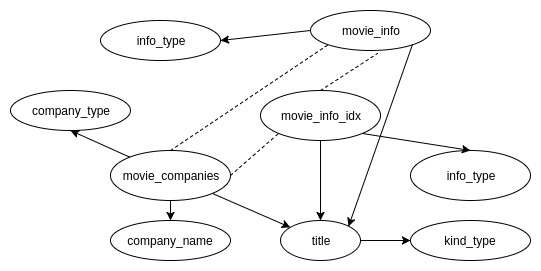
\includegraphics[width=1.0\textwidth]{query_graph_JOB.jpg}
	\caption{Typical query graph of JOB workload \cite{JOB}.}
\end{figure}

\section{CONCLUSION}

Although TPC-H, TPC-E, TPC-DS or the Star Schema Benchmark (SSB) have proven their value for evaluating query engines, I argue
that they are not good bechmark for the cardinality estimation component of query optimizers. The reason is that the data generators
use the assumptions (uniformity, independence, principle of inclusion). These assumptions are the reasons leading to the limitaions of
cardinality estimator of PostgresSQL. However, There are full of correlations and non-uniform data distributions in current real-world 
data sets, which makes cardinality estimation much harder. Therefore, I don't use these benchmarks for benchmarking cardinality estimation
in PostgreSQL.

Besides, JOB benchmark solved the limitation of the benchmarks above. IMDB data set is real-world data set with full of correlations and 
non-uniform data distributions and its queries contain many joins, which makes cardinality estimator of PostgreSQL encounter hardships. So 
it is very suitable to be used for benchmarking cardinality estimation in PostgreSQL.



